% AGENT 2027 (ICSE 2027 workshop on Agentic Engineering) -- short paper.
% Limits: short papers up to 5 pages INCLUDING references; IEEE conference
% template; single-anonymous. Every number is a macro from numbers.tex
% (generated by analysis/paper_numbers.py) or results.tex (generated from
% the measurement results); never type a number by hand.
\documentclass[10pt,conference]{IEEEtran}
\usepackage[T1]{fontenc}
\usepackage[utf8]{inputenc}
\usepackage{graphicx}
\usepackage{booktabs}
\usepackage{pgfplots}
\pgfplotsset{compat=1.18}
\usepackage{xspace}
\usepackage{amsmath}
\usepackage[hidelinks]{hyperref}
\usepackage{orcidlink}
\usepackage[capitalise]{cleveref}
% GENERATED by analysis/paper_numbers.py -- do not edit by hand
\newcommand{\nPop}{361,296\xspace}  % data/p1_counts.json pop_prs (AIDev v5 AIDev-pop)
\newcommand{\nPopRepos}{25,402\xspace}  % data/p1_counts.json pop_repos_rows
\newcommand{\nAllPRs}{7,685,281\xspace}  % data/p1_counts.json all_pull_request rows
\newcommand{\nCand}{108,708\xspace}  % data/p1_keyword_stats.json candidates
\newcommand{\pctCand}{30.1\%\xspace}  % candidates / AIDev-pop
\newcommand{\nPilot}{2,000\xspace}  % pilot_summary_cc.json n
\newcommand{\nPilotLabelled}{1,999\xspace}  % pilot labels status ok
\newcommand{\nPilotRuntime}{465\xspace}  % pilot runtime perf (primary|secondary + runtime)
\newcommand{\pctPilotRuntime}{23.3\%\xspace}  % pilot runtime perf share
\newcommand{\pctPilotNone}{68.9\%\xspace}  % pilot role none share
\newcommand{\nStratClassified}{5,900\xspace}  % p2_classify/summary.json classified
\newcommand{\nRuntimePRs}{1,343\xspace}  % p2_classify/summary.json runtime_perf_total
\newcommand{\nStratHaiku}{4,769\xspace}  % p2 labeller counts
\newcommand{\nStratOpus}{1,130\xspace}  % p2 labeller counts
\newcommand{\haikuKappa}{0.79\xspace}  % p2_haiku_agree/agreement.json runtime_perf_kappa
\newcommand{\haikuAgreeN}{66\xspace}  % agreement n_compared
\newcommand{\haikuAgree}{91\%\xspace}  % agreement runtime_perf_agreement
\newcommand{\nClaims}{1,343\xspace}  % p5_claims/all_v1/claims_pr.parquet ok
\newcommand{\nNoMech}{189\xspace}  % claims: mechanism_stated false
\newcommand{\pctNoMech}{14.1\%\xspace}  % share
\newcommand{\nEffect}{422\xspace}  % claims: claimed_effect non-empty
\newcommand{\pctEffect}{31.4\%\xspace}  % share
\newcommand{\evBenchmark}{221\xspace}  % claims evidence == benchmark
\newcommand{\evTest}{347\xspace}  % claims evidence == test
\newcommand{\evReasoning}{500\xspace}  % claims evidence == reasoning
\newcommand{\evNone}{269\xspace}  % claims evidence == none
\newcommand{\evProfile}{6\xspace}  % claims evidence == profile
\newcommand{\pctReasonNone}{57.3\%\xspace}  % evidence reasoning|none share
\newcommand{\pctBenchmark}{16.5\%\xspace}  % evidence benchmark share
\newcommand{\mechAlgorithmic}{9.5\%\xspace}  % claims_mech: PRs with mechanism algorithmic / nClaims
\newcommand{\mechAsyncIo}{5.5\%\xspace}  % claims_mech: PRs with mechanism async_io / nClaims
\newcommand{\mechAvoidRepeatedIo}{2.6\%\xspace}  % claims_mech: PRs with mechanism avoid_repeated_io / nClaims
\newcommand{\mechBatchCalls}{2.7\%\xspace}  % claims_mech: PRs with mechanism batch_calls / nClaims
\newcommand{\mechCacheResults}{15.3\%\xspace}  % claims_mech: PRs with mechanism cache_results / nClaims
\newcommand{\mechConcurrencyTuning}{4.2\%\xspace}  % claims_mech: PRs with mechanism concurrency_tuning / nClaims
\newcommand{\mechFasterDbQuery}{3.7\%\xspace}  % claims_mech: PRs with mechanism faster_db_query / nClaims
\newcommand{\mechFasterLibrary}{4.2\%\xspace}  % claims_mech: PRs with mechanism faster_library / nClaims
\newcommand{\mechFewerDbQueries}{3.6\%\xspace}  % claims_mech: PRs with mechanism fewer_db_queries / nClaims
\newcommand{\mechFewerExternalCalls}{4.2\%\xspace}  % claims_mech: PRs with mechanism fewer_external_calls / nClaims
\newcommand{\mechFewerProcesses}{0.2\%\xspace}  % claims_mech: PRs with mechanism fewer_processes / nClaims
\newcommand{\mechFewerSyscalls}{0.2\%\xspace}  % claims_mech: PRs with mechanism fewer_syscalls / nClaims
\newcommand{\mechGpuAccelerator}{2.8\%\xspace}  % claims_mech: PRs with mechanism gpu_accelerator / nClaims
\newcommand{\mechIoGranularity}{0.9\%\xspace}  % claims_mech: PRs with mechanism io_granularity / nClaims
\newcommand{\mechLazyLoading}{4.1\%\xspace}  % claims_mech: PRs with mechanism lazy_loading / nClaims
\newcommand{\mechLessLocking}{1.7\%\xspace}  % claims_mech: PRs with mechanism less_locking / nClaims
\newcommand{\mechLessMemory}{16.6\%\xspace}  % claims_mech: PRs with mechanism less_memory / nClaims
\newcommand{\mechLessOutput}{1.5\%\xspace}  % claims_mech: PRs with mechanism less_output / nClaims
\newcommand{\mechOther}{12.1\%\xspace}  % claims_mech: PRs with mechanism other / nClaims
\newcommand{\mechParallelize}{6.9\%\xspace}  % claims_mech: PRs with mechanism parallelize / nClaims
\newcommand{\mechPollingSleep}{2.1\%\xspace}  % claims_mech: PRs with mechanism polling_sleep / nClaims
\newcommand{\mechPrecompute}{5.4\%\xspace}  % claims_mech: PRs with mechanism precompute / nClaims
\newcommand{\mechReuseResources}{3.9\%\xspace}  % claims_mech: PRs with mechanism reuse_resources / nClaims
\newcommand{\mechSkipUnneededWork}{20.6\%\xspace}  % claims_mech: PRs with mechanism skip_unneeded_work / nClaims
\newcommand{\mechSmallerPayload}{2.7\%\xspace}  % claims_mech: PRs with mechanism smaller_payload / nClaims
\newcommand{\mechStreamingOutput}{1.1\%\xspace}  % claims_mech: PRs with mechanism streaming_output / nClaims
\newcommand{\mechUiRendering}{2.1\%\xspace}  % claims_mech: PRs with mechanism ui_rendering / nClaims
\newcommand{\mechVectorizeLocality}{3.3\%\xspace}  % claims_mech: PRs with mechanism vectorize_locality / nClaims
\newcommand{\nMeasurableClaims}{1,030\xspace}  % PRs with >= 1 mechanism outside {gpu, external API, UI, other}
\newcommand{\nQuotes}{2,087\xspace}  % claims_mech rows
\newcommand{\nQuotesNotFound}{46\xspace}  % quotes not found after whitespace normalisation
\newcommand{\nGhError}{19\xspace}  % jobs/_stats.json github_error (repo/PR unavailable)
\newcommand{\nNoPyFinal}{62\xspace}  % jobs/_refilter_stats.json no_py_in_final_diff
\newcommand{\nJobs}{949\xspace}  % jobs/_refilter_stats.json kept
\newcommand{\nVMs}{3\xspace}  % data/p7_paper/vm_controls/*.json
\newcommand{\nControls}{12\xspace}  % controls per VM
\newcommand{\nChecks}{22\xspace}  % expectation checks per VM
\newcommand{\ctrlPassMin}{21\xspace}  % min PASS over VMs
\newcommand{\ctrlPassMax}{22\xspace}  % max PASS over VMs
\newcommand{\nIntegrityProblems}{0\xspace}  % multiplexed counters + lost events/packets, all VMs
\newcommand{\counterErrMax}{3.5\times10^{-5}\xspace}  % max relative error of the exact-instruction check over VMs
\newcommand{\faultRatioMin}{0.888\xspace}  % LTTng page-fault events / perf faults, min over controls+VMs
\newcommand{\faultRatioMed}{0.943\xspace}  % median of the same

% GENERATED by analysis/p7_results.py -- do not edit by hand
\newcommand{\nMeasured}{91\xspace}  % PRs with measure.json (fetched)
\newcommand{\nExcludedReview}{4\xspace}  % excluded in manual review (data/p7_paper/review.json)
\newcommand{\nExcludedIntegrity}{0\xspace}  % multiplexed/lost events
\newcommand{\nExcludedNoisy}{1\xspace}  % A/A wall ratio outside 0.95-1.05
\newcommand{\nAnalysed}{82\xspace}  % measured, clean, >=1 checkable claimed mechanism, Python >= 50% of change
\newcommand{\nReposAnalysed}{53\xspace}  % distinct repositories in nAnalysed
\newcommand{\maxPerRepo}{15\xspace}  % PRs of the most frequent repository
\newcommand{\topRepo}{iPhotron-LocalPhotoAlbumManager\xspace}  % most frequent repository
\newcommand{\nFaster}{32\xspace}  % speed == faster
\newcommand{\nSlower}{22\xspace}  % speed == slower
\newcommand{\nNoChange}{28\xspace}  % speed == no_change
\newcommand{\nHeld}{34\xspace}  % any claimed mechanism signal moved as claimed
\newcommand{\qFH}{28\xspace}  % speed faster & held True
\newcommand{\qFN}{4\xspace}  % speed faster & held False
\newcommand{\qNH}{3\xspace}  % speed no_change & held True
\newcommand{\qNN}{25\xspace}  % speed no_change & held False
\newcommand{\qSH}{3\xspace}  % speed slower & held True
\newcommand{\qSN}{19\xspace}  % speed slower & held False
\newcommand{\nBehaviour}{42\xspace}  % output digest differs base vs head
\newcommand{\nHiddenCost}{21\xspace}  % any cost signal up >= 10%, separated
\newcommand{\nHiddenCostFaster}{3\xspace}  % hidden cost among faster PRs
\newcommand{\aaMin}{0.965\xspace}  % min A/A wall ratio
\newcommand{\aaMax}{1.009\xspace}  % max A/A wall ratio
\newcommand{\nLowPy}{4\xspace}  % clean measured PRs with Python < 50% of change
\newcommand{\nAttempted}{150\xspace}  % build verdicts (real outcomes; usage-limit failures excluded)
\newcommand{\funChangeUnreachable}{2\xspace}  % funnel: change_unreachable
\newcommand{\funFailedCheck}{16\xspace}  % funnel: failed_check
\newcommand{\funInstallFailed}{2\xspace}  % funnel: install_failed
\newcommand{\funNeedsExternalService}{13\xspace}  % funnel: needs_external_service
\newcommand{\funNeedsGpu}{4\xspace}  % funnel: needs_gpu
\newcommand{\funNewCodeOnly}{14\xspace}  % funnel: new_code_only
\newcommand{\funNotPythonChange}{6\xspace}  % funnel: not_python_change
\newcommand{\funOther}{2\xspace}  % funnel: other
\newcommand{\funPassed}{91\xspace}  % funnel: passed
\newcommand{\pctPassed}{61\%\xspace}  % passed / attempted
\newcommand{\usdPerBuild}{\$0.37\xspace}  % mean list-price-equivalent agent cost per build

% generated by analysis/p7_cases.py; do not edit
\newcommand{\caseAWall}{0.88$\times$}
\newcommand{\caseAWallBase}{2.60}
\newcommand{\caseAWallHead}{2.28}
\newcommand{\caseASys}{1.41$\times$}
\newcommand{\caseASysBase}{0.18}
\newcommand{\caseASysHead}{0.26}
\newcommand{\caseASyscalls}{3.49$\times$}
\newcommand{\caseASyscallsBase}{74,797}
\newcommand{\caseASyscallsHead}{261,258}
\newcommand{\caseAPread}{11.56$\times$}
\newcommand{\caseAPreadBase}{1,132}
\newcommand{\caseAPreadHead}{13,089}
\newcommand{\caseABytes}{2.47$\times$}
\newcommand{\caseABytesBase}{23,278,166}
\newcommand{\caseABytesHead}{57,387,870}
\newcommand{\caseATask}{1.32$\times$}
\newcommand{\caseATaskBase}{1,607}
\newcommand{\caseATaskHead}{2,114}
\newcommand{\caseAThreads}{1.68$\times$}
\newcommand{\caseAThreadsBase}{19}
\newcommand{\caseAThreadsHead}{32}
\newcommand{\caseBWall}{11.35$\times$}
\newcommand{\caseBWallBase}{0.90}
\newcommand{\caseBWallHead}{10.19}
\newcommand{\caseBGetdents}{41.82$\times$}
\newcommand{\caseBGetdentsBase}{294}
\newcommand{\caseBGetdentsHead}{12,294}
\newcommand{\caseBInstr}{17.88$\times$}
\newcommand{\caseBInstrBase}{6,253,905,490}
\newcommand{\caseBInstrHead}{111,799,447,031}
\newcommand{\caseCWall}{0.82$\times$}
\newcommand{\caseCWallBase}{2.55}
\newcommand{\caseCWallHead}{2.09}
\newcommand{\caseCRead}{0.24$\times$}
\newcommand{\caseCReadBase}{17,215}
\newcommand{\caseCReadHead}{4,063}
\newcommand{\caseCInstr}{0.73$\times$}
\newcommand{\caseCInstrBase}{25,910,100,695}
\newcommand{\caseCInstrHead}{18,820,510,383}
\newcommand{\caseDWall}{1.47$\times$}
\newcommand{\caseDWallBase}{4.32}
\newcommand{\caseDWallHead}{6.32}
\newcommand{\caseDOffcpu}{0.87$\times$}
\newcommand{\caseDOffcpuBase}{1,131,051,365}
\newcommand{\caseDOffcpuHead}{978,737,838}
\newcommand{\caseDSyscalls}{2.16$\times$}
\newcommand{\caseDSyscallsBase}{87,007}
\newcommand{\caseDSyscallsHead}{187,552}
\newcommand{\caseDFutexc}{2.86$\times$}
\newcommand{\caseDFutexcBase}{119}
\newcommand{\caseDFutexcHead}{340}
\newcommand{\caseDTask}{1.43$\times$}
\newcommand{\caseDTaskBase}{4,298}
\newcommand{\caseDTaskHead}{6,156}
\newcommand{\caseDSocket}{1.00$\times$}
\newcommand{\caseDSocketBase}{6}
\newcommand{\caseDSocketHead}{6}
\newcommand{\caseDConnect}{1.00$\times$}
\newcommand{\caseDConnectBase}{4}
\newcommand{\caseDConnectHead}{4}

\newcommand{\sys}{\textsc{Below}\xspace}

\begin{document}
\title{Below the Stopwatch: Checking the Performance Claims of Coding Agents in the Kernel}

% Author block given by the user on 2026-11-20 (two centred rows of two).
\author{
\IEEEauthorblockN{Yuvraj Sehgal\,\orcidlink{0009-0002-1980-604X}}
\IEEEauthorblockA{\textit{Department of Computer Science}\\
\textit{Brock University}\\
St.\ Catharines, Ontario, Canada\\
ys19rk@brocku.ca}
\and[\hspace{0.6in}]
\IEEEauthorblockN{Sneh Patel\,\orcidlink{0000-0002-1985-8715}}
\IEEEauthorblockA{\textit{Department of Computer Science}\\
\textit{Brock University}\\
St.\ Catharines, Ontario, Canada\\
sp18oo@brocku.ca}
\and[\hfill\vspace{1em}\break\hspace*{\fill}]
\IEEEauthorblockN{Mahsa Panahandeh\,\orcidlink{0000-0002-6369-8982}}
\IEEEauthorblockA{\textit{School of Electrical Engineering}\\
\textit{and Computer Science}\\
\textit{University of Ottawa}\\
Ottawa, Ontario, Canada\\
mpanahan@uottawa.ca}
\and[\hspace{0.6in}]
\IEEEauthorblockN{Naser Ezzati-Jivan\,\orcidlink{0000-0003-1435-6297}}
\IEEEauthorblockA{\textit{Department of Computer Science}\\
\textit{Brock University}\\
St.\ Catharines, Ontario, Canada\\
nezzatijivan@brocku.ca}
}

\maketitle

\begin{abstract}
Coding agents open many pull requests that claim to make software faster.
Prior studies read these claims or re-execute a few of them; a stopwatch shows
whether code got faster, but not whether it got faster for the reason the
agent gives. We check agents' performance claims at the kernel level. From
\nRuntimePRs runtime-performance pull requests in the AIDev dataset we
extract the mechanism each one claims, map it to the kernel and hardware
signals that must move if the claim is true, rebuild both versions with a
build agent that never sees the claim, and measure them with untraced
timing, hardware counters and LTTng kernel traces. Agents rarely back their
claims: \pctReasonNone offer only reasoning or no evidence, and
\pctEffect state any effect size. In first measurements of \nAnalysed PRs,
\nFaster ran faster, \nNoChange showed no clear change and \nSlower ran
slower; the claimed mechanism left its kernel footprint in \nHeld, and
\nBehaviour also changed their output. Kernel signals separate claimed
from unclaimed mechanisms far better than the instruction count
(\kRatioFast$\times$ against \iRatioFast$\times$ for faster PRs), showing
what looking below the stopwatch adds.

\end{abstract}

\section{Introduction}
\label{sec:intro}

Coding agents now open pull requests (PRs) at scale: the AIDev dataset
alone records \nAllPRs agent-authored PRs from six agents~\cite{li2026aidev}.
Many of these PRs claim to make software faster or lighter. Studies of such
performance PRs read their text~\cite{opu2025bertopic,peng2025optimization,
dovhoshliubnyi2026mutation,peng2026validation} or, at most, re-execute a
few dozen of them~\cite{qi2026merged}. They find that agents rely more on
static reasoning and less on benchmarks than humans
do~\cite{peng2026validation}, and that re-executed claims often do not
hold~\cite{qi2026merged}.

A stopwatch answers whether a change is faster, not \emph{why}. Yet a
performance PR usually claims a mechanism: \emph{cache the result},
\emph{read the file once}, \emph{stream in 1\,MB chunks}, \emph{remove the
lock}. Each mechanism leaves a footprint in the operating system: fewer
\texttt{read} calls, fewer page faults, less time waiting on a futex. If
the footprint is absent, the claim is wrong even when the code is faster;
if it is present but the code is not faster, the mechanism was not the
bottleneck. Neither case is visible to a stopwatch.

We present \sys, a method and pipeline that checks agents' performance
claims at the kernel level. It (i)~finds performance PRs and extracts the
mechanism each one claims, (ii)~maps each mechanism to the kernel and
hardware signals that must move if the claim is true, (iii)~uses a
\emph{blind} build agent to rebuild the code before and after each PR and
write a workload that runs the changed code, and (iv)~measures both
versions with untraced timing, hardware counters and full LTTng kernel
traces~\cite{desnoyers2006lttng}. This short paper reports the method, its
validation, a characterization of \nClaims agent performance claims, and
first measurement results.

\section{Approach}
\label{sec:approach}

\begin{figure*}[t]
\centering
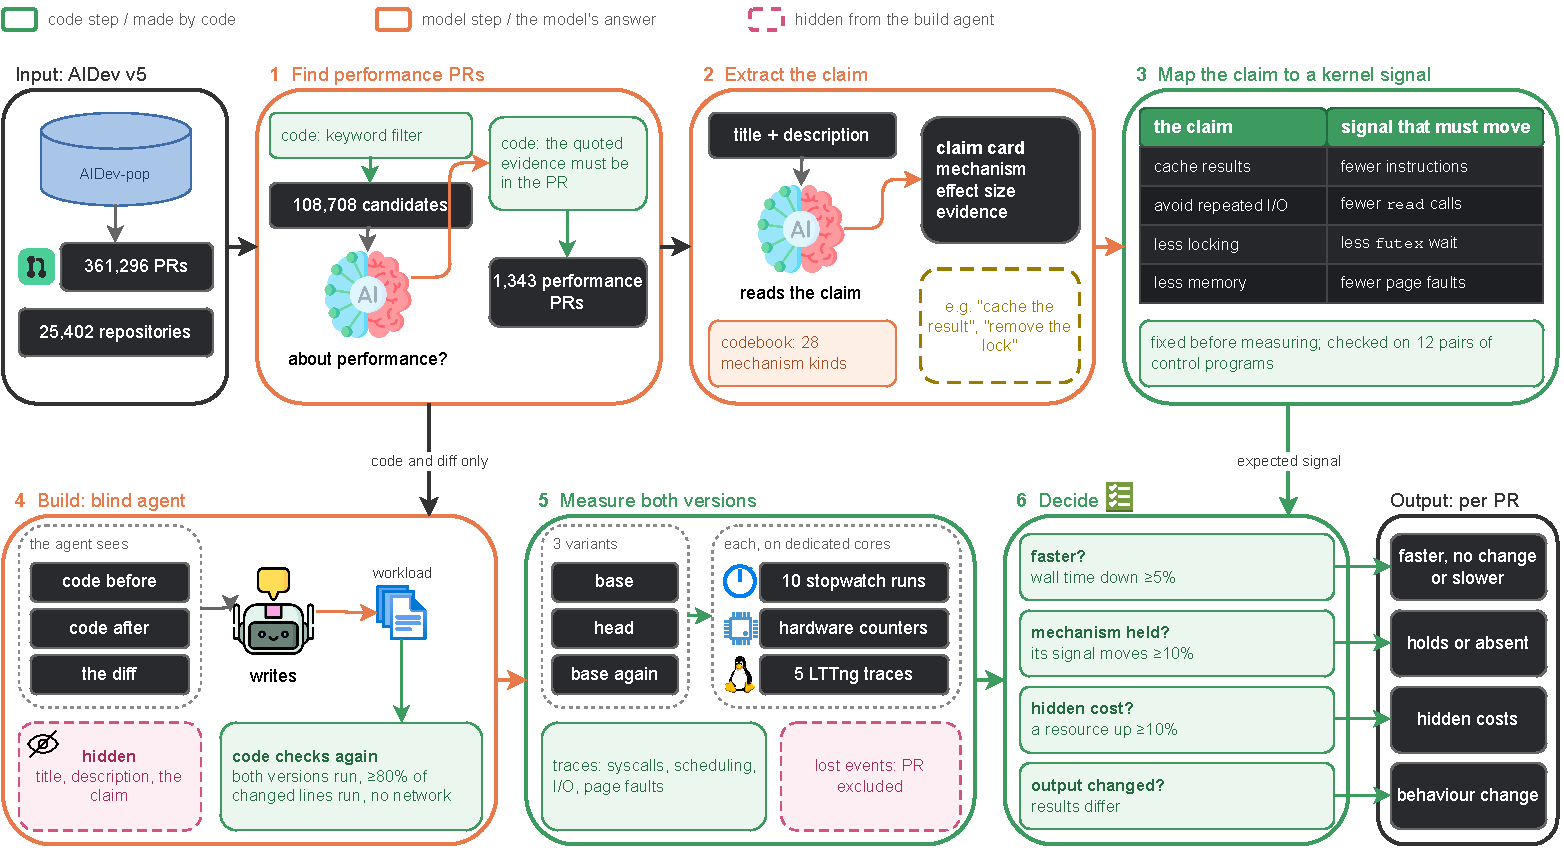
\includegraphics[width=\textwidth]{figures/final.pdf}
\caption{Overview of \sys. Orange boxes are model steps and green boxes
are code. The build agent (step~4) sees only the code and the diff; the
PR text and the claim are hidden from it (pink). The expected signal from
step~3 goes straight to the decision in step~6.}
\label{fig:overview}
\end{figure*}

Figure~\ref{fig:overview} shows the six steps of the pipeline.

\subsection{Performance PRs and their claims}
\label{sec:data}
We use AIDev~\cite{li2026aidev} (version~5, pinned to one dataset commit),
restricted to its \emph{AIDev-pop} subset of \nPop agent PRs from
\nPopRepos repositories with more than 100 stars. A keyword filter over
titles, bodies and commit messages (after removing per-agent template
text) keeps \nCand candidates (\pctCand). An LLM classifier with a written
codebook labels whether a PR's goal is to make the software run faster or
use fewer resources; on a random sample of \nPilot candidates,
\pctPilotRuntime are runtime-performance PRs and \pctPilotNone are not
about performance at all. A stratified run over candidates that change
Python code (fixed random order per agent, with a stop rule per agent)
classifies \nStratClassified PRs and yields \nRuntimePRs runtime-performance
PRs. Labels come from Claude Opus~5.5 (\nStratOpus PRs) and, to save cost,
Claude Haiku~5.5 (\nStratHaiku PRs); on \haikuAgreeN PRs labelled by both,
they agree on \haikuAgree (Cohen's $\kappa=\haikuKappa$). Every label
must quote its evidence verbatim from the PR; code checks the quote.

A second codebook, revised once after open coding of 100 PRs and then
frozen, extracts from each runtime-performance PR the mechanism(s) it
claims (28 categories), the claimed effect size, and the evidence it
offers (Table~\ref{tab:oracle} lists the measurable mechanisms).

\subsection{From claimed mechanism to kernel signal}
\label{sec:oracle}
Each mechanism is mapped, before any measurement, to the signals that must
move if the claim is true (Table~\ref{tab:oracle}). Twelve pairs of small
control programs, one pair per signal family, show that each signal moves
as designed: e.g.\ reading a file 2,000 times instead of once, or a
two-thread mutex against per-thread counters.

\begin{table}[t]
\caption{Claimed mechanism, share of the \nClaims runtime-performance PRs
that claim it (a PR may claim several), and the signal that must move.}
\label{tab:oracle}
\centering\scriptsize
\setlength{\tabcolsep}{3pt}
\begin{tabular}{@{}lrl@{}}
\toprule
mechanism claimed & PRs & signal (head vs.\ base) \\
\midrule
skip unneeded work & \mechSkipUnneededWork & fewer syscalls / instructions \\
less memory, fewer copies & \mechLessMemory & fewer page faults, page allocations \\
cache results & \mechCacheResults & fewer instructions (and syscalls) \\
algorithmic & \mechAlgorithmic & fewer instructions, syscalls unchanged \\
parallelize & \mechParallelize & wall time down, CPU time not down \\
async / non-blocking I/O & \mechAsyncIo & less off-CPU time on the main thread \\
precompute & \mechPrecompute & fewer instructions on the hot path \\
faster library & \mechFasterLibrary & fewer instructions \\
concurrency tuning & \mechConcurrencyTuning & threads, context switches, futex \\
lazy loading & \mechLazyLoading & fewer \texttt{openat} / bytes read \\
reuse resources & \mechReuseResources & fewer \texttt{socket}/\texttt{connect}/\texttt{clone} \\
DB: faster / fewer queries & \mechFasterDbQuery\,/\,\mechFewerDbQueries & fewer page reads, round trips \\
vectorize, locality & \mechVectorizeLocality & fewer instructions, cache misses \\
avoid repeated I/O & \mechAvoidRepeatedIo & fewer \texttt{openat}/\texttt{read}, bytes \\
less locking & \mechLessLocking & less futex wait \\
\bottomrule
\end{tabular}
\end{table}

\subsection{Blind build agent and measurement}
\label{sec:harness}
For each PR, the harness checks out the merge base and the PR head (the
API's base commit can be later than the branch point and would mix in
unrelated changes), installs both with dependencies frozen at the PR's
creation date, and hands them to a build agent (Claude Code, Opus~5.5).
The agent is \emph{blind to the claim}: it sees the code, the diff and the
changed files, but not the title, description, commit messages or our
extracted claim, and the git history is moved out of its reach. It must
write a deterministic workload that runs the changed code on both
versions, may stub only external I/O, and must not patch the code under
test. The harness then re-checks independently: both versions run, the
workload executes at least 80\% of the executable lines the PR adds or
changes (50\% for PRs with over 200 such lines), the base version runs 0.5--30\,s, the
workload runs without a network, and the two output digests are compared.
Transcripts are audited for access to the PR on GitHub.

Measurements run on \nVMs identical Google Cloud C4 virtual machines with
the performance-monitoring unit enabled, one job per machine at a time.
Workloads run on dedicated cores (one, or two for parallel workloads):
system services are confined to the other cores with systemd, because \texttt{isolcpus} disables load balancing
(a two-process pool ran on a single core). Per PR we run base, head and
base again (an A/A control): 3+3 warm-up runs, 10 untraced timing runs per
variant, 5 runs of 3 hardware-counter groups (at most four programmable
events each, so no counter is multiplexed), and 5 full LTTng kernel traces
per variant (all syscalls, scheduling, block I/O, interrupts, page faults,
page allocation), filtered to the workload's process tree and with per-file
I/O attribution. PRs with any lost trace events or multiplexed counters are excluded from
the analysis. On each machine,
the \nControls control pairs pass \ctrlPassMin--\ctrlPassMax of \nChecks
checks; the only failure is context switches under lock contention, a
non-deterministic signal whose primary signal (\texttt{futex}) passes. An
exact-instruction loop is counted within a relative error of
$\counterErrMax$, and LTTng's page-fault events agree with perf's fault
counter at a median ratio of \faultRatioMed.

\section{Results}
\label{sec:results}

\subsection{What agents claim, and how they back it}
\label{sec:claims}
Of the \nClaims runtime-performance PRs, \nNoMech (\pctNoMech) name no
mechanism at all. The most common mechanisms are skipping unneeded work
(\mechSkipUnneededWork), reducing memory use or copies (\mechLessMemory)
and caching results (\mechCacheResults) (Table~\ref{tab:oracle}). Claims
are rarely measured: \evReasoning PRs support the claim by reasoning only
and \evNone offer no evidence (together \pctReasonNone); \evBenchmark cite
a benchmark (\pctBenchmark), \evTest a test, and \evProfile a profile. Only
\nEffect (\pctEffect) state an effect size. \nMeasurableClaims PRs claim
at least one mechanism with a kernel or hardware signal; the rest claim
only GPU, external-API, user-interface or uncategorized mechanisms, or
none.

\subsection{Building the PRs}
\label{sec:funnel}
Of the \nMeasurableClaims PRs, \nGhError are no longer available on GitHub
and \nNoPyFinal do not change Python code in their final diff (AIDev's
per-commit file lists include commits merged in from the base branch),
leaving \nJobs build jobs in one fixed random order. In the first batch
(the first \nAttempted of that order), the build agent produced a
workload that passed the harness checks for \funPassed of \nAttempted
attempted PRs (\pctPassed), at about \usdPerBuild per PR. The others need
an external service (\funNeedsExternalService), add only new code that the
base version cannot run (\funNewCodeOnly), need a GPU (\funNeedsGpu), failed
to install (\funInstallFailed), had unreachable changed code
(\funChangeUnreachable), or did not change Python in a runnable way
(\funNotPythonChange); for \funFailedCheck the agent reported success but
the independent check failed, and \funOther could not be classified.

\subsection{Do the claims hold below the stopwatch?}
\label{sec:measure}
We analyse the \nAnalysed measured PRs (from \nReposAnalysed repositories)
whose claim names at least one checkable mechanism and whose change is
mostly Python; \nLowPy measured PRs whose change is mostly non-Python code
are set aside, because their claim may concern code we do not execute.
The manual review excludes \nExcludedReview PRs: in three the claimed
mechanism lies in code the workload never runs, and in one the base
version fails on the measured path. \nExcludedNoisy PR is excluded because its A/A control (base against base)
itself differs by more than 5\%; for the others the A/A wall-time ratio
stays within \aaMin--\aaMax, so the noise floor is small. A PR is \emph{faster} if its
median wall time drops by at least 5\% and every head run is faster than
every base run; a mechanism \emph{holds} if one of its signals
(Table~\ref{tab:oracle}) moves by at least 10\% in the claimed direction
with complete separation between head and base runs.

\begin{table}[t]
\caption{First measurements: wall time against the claimed mechanism, for
the \nAnalysed analysed PRs.}
\label{tab:quadrant}
\centering\footnotesize
\begin{tabular}{@{}lccc@{}}
\toprule
 & faster & no clear change & slower \\
\midrule
claimed mechanism holds & \qFH & \qNH & \qSH \\
claimed mechanism absent & \qFN & \qNN & \qSN \\
\bottomrule
\end{tabular}
\end{table}

\begin{figure}[t]
\centering
\begin{tikzpicture}
\begin{semilogxaxis}[width=\columnwidth, height=4.2cm,
  xlabel={wall time, head / base (log scale)}, ylabel={PR (sorted)},
  ytick=\empty, xmin=0.03, xmax=15, enlarge y limits=0.07,
  xtick={0.05,0.1,0.2,0.5,1,2,5,10}, xticklabels={0.05,0.1,0.2,0.5,1,2,5,10},
  legend style={font=\scriptsize, at={(0.98,0.04)}, anchor=south east},
  label style={font=\footnotesize}, tick label style={font=\footnotesize}]
\fill[gray!20] ({axis cs:0.95,1}|-{rel axis cs:0,0}) rectangle ({axis cs:1.05,1}|-{rel axis cs:0,1});
\draw[gray] ({axis cs:1,1}|-{rel axis cs:0,0}) -- ({axis cs:1,1}|-{rel axis cs:0,1});
\addplot[only marks, mark=*, black] table[x=ratio, y=rank,
  restrict expr to domain={\thisrow{held}}{1:1}] {fig_wall.dat};
\addplot[only marks, mark=o, black] table[x=ratio, y=rank,
  restrict expr to domain={\thisrow{held}}{0:0}] {fig_wall.dat};
\legend{mechanism holds, mechanism absent}
\end{semilogxaxis}
\end{tikzpicture}
\caption{Wall-time ratio of each analysed PR. The grey band is the
$\pm$5\% zone counted as no clear change.}
\label{fig:wall}
\end{figure}

Table~\ref{tab:quadrant} and Figure~\ref{fig:wall} show the first results. Of the \nAnalysed PRs,
\nFaster are faster, \nNoChange show no clear change and \nSlower are
slower than before the change; the claimed mechanism holds in \nHeld.
When a PR is faster, its claimed mechanism usually appears (\qFH of
\nFaster); when it is slower, it rarely does (\qSH of \nSlower). In this
sample, a missing footprint rarely comes with a speed-up. The rule does not
fire by chance: applied to base against base again, it moves none of
\aaSigTests signal tests (\aaSigRate). It is, however, only partly
specific, because several mechanisms share the instruction count: for the
faster PRs, the signals of mechanisms a PR did \emph{not} claim also move
in \spUnclaimedRateFast of cases, against \spClaimedRateFast for the
claimed ones. A held mechanism is therefore evidence consistent with the
claim, not proof of it.
\nBehaviour PRs also change the output of the workload (for example new
defaults or error messages), as Qi et al.\ also observe for merged agent
fixes~\cite{qi2026merged}. The pattern is the same with and without such
changes: of the \nSame PRs whose output is unchanged, \qFHSame are faster
with the mechanism present and \qFNSame faster without it. \nHiddenCost
PRs make at least one resource clearly worse (system time, memory, page faults, syscalls,
instructions, CPU time or bytes read).

% Case studies. Every number is a macro from analysis/p7_cases.py, which
% reads the medians of the measured runs and asserts full separation.
\paragraph{Faster, but not for the claimed reason}
iPhotron PR~\#453 (Copilot) claims to remove the slowdown of deep SQL
pagination and to load assets on demand instead of all at once. The workload
runs \caseAWall\ of the base wall time (\caseAWallBase\,s to
\caseAWallHead\,s; all ratios use unrounded medians), yet the kernel shows more work, not less: \caseASyscalls\
the syscalls (\caseASyscallsBase\ to \caseASyscallsHead), \caseAPread\ the
\texttt{pread64} calls, \caseABytes\ the bytes read and \caseASys\ the system
time. Total CPU time grows \caseATask\ while the process runs
\caseAThreadsHead\ threads instead of \caseAThreadsBase. Peak memory does not
change. A stopwatch would credit the claim; the trace does not support it.

\paragraph{Slower, and the trace shows where}
iPhotron PR~\#564 (Jules) uses pre-generated thumbnails. On our workload,
which keeps 500 unrelated files in the thumbnail folder, it is
\caseBWall\ slower (\caseBWallBase\,s to \caseBWallHead\,s) and its output
changes. The trace shows a likely cause: \texttt{getdents64}, the call that
lists a directory, rises from \caseBGetdentsBase\ to \caseBGetdentsHead\
(\caseBGetdents), and instructions grow \caseBInstr.

\paragraph{Half the mechanism happens, and it hurts}
A Claude Code PR to gemini-notebook-mcp-cli (\#16) claims non-blocking
I/O and HTTP connection pooling. The first part appears: the main thread
spends \caseDOffcpu\ of its former time off the CPU. The second does not:
the workload opens \caseDSocketHead\ sockets and \caseDConnectHead\
connections on both versions. Meanwhile syscalls grow \caseDSyscalls,
\texttt{futex} calls \caseDFutexc\ and CPU time \caseDTask, and the
workload is \caseDWall\ slower (\caseDWallBase\,s to \caseDWallHead\,s).

\paragraph{A claim that holds}
mlflow PR~\#19520 (Copilot) changes artifact transfer to chunked streaming.
The footprint is exactly the claimed one: \texttt{read} calls fall from
\caseCReadBase\ to \caseCReadHead\ (\caseCRead) for the same bytes read,
instructions fall to \caseCInstr\ and wall time to \caseCWall\ of the base.


\section{Discussion, threats and related work}
\label{sec:discussion}

\textbf{What this means for agent builders and reviewers.} A performance
PR whose mechanism leaves no kernel footprint, or whose speed-up comes with
a changed output, should not be merged on its description. Kernel signals
are cheap to collect once a workload exists; asking agents to attach the
trace evidence for the mechanism they claim would turn many unverifiable
claims into checkable ones.

\textbf{Threats to validity.} The measured sample is small and early
(\nAnalysed PRs, up to \maxPerRepo from one repository), so the shares in
Table~\ref{tab:quadrant} are preliminary. Workloads are written by an
agent: although it never sees the claim and an independent check enforces
coverage of the changed lines, a workload may not reflect real use. Because
the agent is blind to the claim, it may exercise a different part of a
large PR than the one the claim is about; the review removed such PRs when
it found them, but others may remain and would bias towards
``mechanism absent''.
Classification and claim extraction are done by LLMs; a human check of a
stratified sample of 300 PRs is prepared but not yet done. Kernel signals are evidence for a
mechanism, not proof; the control programs show that each signal responds
as expected. Each PR is measured once on one machine; repeated measurements on a
second machine may be added later.

\textbf{Related work.} Studies of agent performance PRs
characterize topics~\cite{opu2025bertopic}, optimization
patterns~\cite{peng2025optimization}, mutation
patterns~\cite{dovhoshliubnyi2026mutation} and how agents report
validation~\cite{peng2026validation}, all from text and code. Qi et
al.\ re-execute 53 fixes from AIDev~\cite{qi2026merged}. Gong et al.\
find agent PR descriptions that claim changes the code does not
implement~\cite{gong2026inconsistency}; we check a claim's runtime
effect instead of its presence in the diff. Benchmarks
such as PIE~\cite{shypula2024pie}, EffiBench~\cite{huang2024effibench},
SWE-Perf~\cite{he2025sweperf}, GSO~\cite{shetty2025gso},
PerfBench~\cite{garg2025perfbench}, SWE-fficiency~\cite{ma2025swefficiency}
and FormulaCode~\cite{sehgal2026formulacode} measure whether models or
agents can make given code faster, and their reliability has been
questioned~\cite{chen2026benchmarks}. Performance bugs in human-written
code have long been studied~\cite{jin2012perfbugs,zaman2012perfbugs}, and
kernel traces have been used to explain where execution time
goes~\cite{giraldeau2016wait,ezzatijivan2017multiscale}. We instead check,
with kernel traces, the mechanism that agent PRs claim.

\textbf{Conclusion.} Agents' performance claims are mostly unmeasured, and
a stopwatch cannot tell whether they are true for the stated reason. Our
pipeline checks the claimed mechanism in the kernel; the full study is
under way on \nJobs PRs.


\section*{Acknowledgment}
In line with the workshop's policy, we disclose substantive use of AI.
Claude models classified the PRs and extracted the claims, and a Claude
Code build agent wrote the workloads. Claude also helped write the
analysis code, summarize related work, prepare the figures and draft this
paper. All numbers are generated from the result files by scripts. Each
measured PR was reviewed before inclusion, and the authors take
responsibility for all content.


\bibliographystyle{IEEEtran}
\bibliography{refs}
\end{document}
